
\includegraphics{src/img/imagine.png}

\hypertarget{connexion}{%
\section{Connexion}\label{connexion}}

Nom de domaine et port SSH sur: \url{http://srvz-webapp2.he-arc.ch/}.

\begin{otherlanguage}{english}

\begin{Shaded}
\begin{Highlighting}[]
\CommentTok{# Exemple}

\NormalTok{$ }\FunctionTok{ssh}\NormalTok{ -p 2030 yoan@srvz-webapp2.he-arc.ch}
\ExtensionTok{yoan@yoan}\NormalTok{$ more ~/README.md}
\end{Highlighting}
\end{Shaded}

\end{otherlanguage}

\hypertarget{mise-uxe0-jour-de-rails}{%
\subsection{Mise à jour de Rails}\label{mise-uxe0-jour-de-rails}}

\begin{otherlanguage}{english}

\begin{Shaded}
\begin{Highlighting}[]
\ExtensionTok{yoan@yoan}\NormalTok{$ rails -v}
\ExtensionTok{Rails}\NormalTok{ 5.0.0.1}
\ExtensionTok{yoan@yoan}\NormalTok{$ gem update}
\ExtensionTok{Updating}\NormalTok{ installed gems}
\ExtensionTok{...}
\ExtensionTok{yoan@yoan}\NormalTok{$ rails -v}
\ExtensionTok{Rails}\NormalTok{ 5.0.1}
\end{Highlighting}
\end{Shaded}

\end{otherlanguage}

\hypertarget{une-application-ruby}{%
\subsection{Une application Ruby}\label{une-application-ruby}}

Comme pour Laravel, c'est une bonne pratique d'avoir un répertoire pour
le contenu publiable sur Internet.

\begin{otherlanguage}{english}

\begin{verbatim}
$ cd /var/www/app
$ ls
config.ru
Gemfile
Gemfile.lock
public/nginx-puma.png

$ more config.ru
\end{verbatim}

\end{otherlanguage}

\hypertarget{rack-101}{%
\section{Rack 101}\label{rack-101}}

\begin{otherlanguage}{english}

\begin{Shaded}
\begin{Highlighting}[]
\NormalTok{run ->(env) }\KeywordTok{do}
\NormalTok{  [}
    \DecValTok{200}\NormalTok{,}
\NormalTok{    \{}\StringTok{"Content-Type"}\NormalTok{ => }\StringTok{"text/html; charset=utf-8"}\NormalTok{\},}
\NormalTok{    [}
      \StringTok{"<!DOCTYPE html>"}\NormalTok{,}
      \StringTok{"<meta charset=utf-8>"}\NormalTok{,}
      \StringTok{"<title>Hello!</title>"}\NormalTok{,}
      \StringTok{"<h1>Hello</h1>"}\NormalTok{,}
      \StringTok{"<p>:-)"}
\NormalTok{    ]}
\NormalTok{  ]}
\KeywordTok{end}
\end{Highlighting}
\end{Shaded}

\end{otherlanguage}

Une fonction, Proc ou lambda qui :

\begin{itemize}
\tightlist
\item
  reçoit un tableau associatif de son environement;
\item
  retourne un triplet de réponse HTTP.
\end{itemize}

Réponse HTTP:

\begin{itemize}
\tightlist
\item
  le code HTTP;
\item
  un tableau associatif des entêtes HTTP;
\item
  un itérateur sur le corps du document.
\end{itemize}

\hypertarget{gemfile}{%
\subsection{\texorpdfstring{\emph{Gemfile}}{Gemfile}}\label{gemfile}}

Un paquet Ruby se nomme une \emph{gemme}.

\begin{otherlanguage}{english}

\begin{Shaded}
\begin{Highlighting}[]
\CommentTok{# Gemfile}
\NormalTok{source }\StringTok{"https://rubygems.org"}

\NormalTok{gem }\StringTok{"puma"}\NormalTok{, }\StringTok{"~> 3.6.2"}
\NormalTok{gem }\StringTok{"rack"}
\end{Highlighting}
\end{Shaded}

\end{otherlanguage}

Comme le composer.json pour PHP.

\hypertarget{nginx}{%
\subsection{NGINX}\label{nginx}}

\begin{otherlanguage}{english}

\begin{verbatim}
root /var/www/app/public;

location / {
    try_files $uri/index.html $uri @rack;
}

location @rack {
    proxy_pass http://puma;
    proxy_set_header X-Forwarded-For $proxy_add_x_forwarded_for;
    proxy_set_header Host $http_host;
    proxy_redirect off;
}

upstream puma {
    server unix:/tmp/puma.sock fail_timeout=0;
}
\end{verbatim}

\end{otherlanguage}

Le serveur HTTP qui sert les fichiers statiques (public) et redirige le
reste vers le serveur d'application Ruby (puma).

\hypertarget{puma}{%
\subsection{Puma}\label{puma}}

Le serveur d'application pour Ruby.

\begin{otherlanguage}{english}

\begin{Shaded}
\begin{Highlighting}[]
\KeywordTok{#!/usr/bin/env puma}

\NormalTok{environment }\StringTok{"production"}

\NormalTok{directory }\StringTok{"/var/www/app"}
\NormalTok{bind }\StringTok{"unix:///tmp/puma.sock"}

\CommentTok{# À ajouter.}
\NormalTok{plugin }\StringTok{:tmp_restart}
\end{Highlighting}
\end{Shaded}

\end{otherlanguage}

En PHP, nous utilisions PHP-FPM. Qu'utilisez-vous avec JEE?

\hypertarget{serveur}{%
\subsection{Serveur}\label{serveur}}

\begin{otherlanguage}{english}

\begin{Shaded}
\begin{Highlighting}[]
\NormalTok{$ }\FunctionTok{ls}\NormalTok{ /etc/services}
\ExtensionTok{cron}\NormalTok{ nginx puma sshd syslog}

\NormalTok{$ }\FunctionTok{pstree}
\ExtensionTok{tini}\NormalTok{───runsvdir─┬─runsv───cron}
\NormalTok{                ├─}\ExtensionTok{runsv}\NormalTok{───nginx───4*[nginx]}
\NormalTok{                ├─}\ExtensionTok{runsv}\NormalTok{───syslog-ng}
\NormalTok{                └─}\ExtensionTok{runsv}\NormalTok{───bundle─┬─}\DataTypeTok{\{reactor.rb:151\}}
\NormalTok{                                 ├─}\DataTypeTok{\{ruby-timer-thr\}}
\NormalTok{                                 ├─}\DataTypeTok{\{server.rb:301\}}
\NormalTok{                                 └─}\ExtensionTok{6*}\NormalTok{[}\DataTypeTok{\{thread_pool.rb*\}}\NormalTok{]}
\end{Highlighting}
\end{Shaded}

\end{otherlanguage}

\hypertarget{exercice-1}{%
\section{Exercice 1}\label{exercice-1}}

Modifiez l'environnement \emph{puma} en
\begin{otherlanguage}{english}\texttt{development}\end{otherlanguage}.

\begin{otherlanguage}{english}\texttt{http://{[}\ PRENOM.NOM\ \textbar{}\ GITHUB\ {]}.srvz-webapp2.he-arc.ch/}\end{otherlanguage}
doit afficher:

\begin{otherlanguage}{english}

\begin{verbatim}
RACK_ENV
    development
\end{verbatim}

\end{otherlanguage}

\hypertarget{premiuxe8re-application}{%
\section{Première application}\label{premiuxe8re-application}}

Archivez \begin{otherlanguage}{english}\texttt{app}\end{otherlanguage}.

\begin{otherlanguage}{english}

\begin{Shaded}
\begin{Highlighting}[]
\NormalTok{$ }\BuiltInTok{cd}\NormalTok{ /var/www}
\NormalTok{$ }\FunctionTok{mv}\NormalTok{ app demoapp}
\end{Highlighting}
\end{Shaded}

\end{otherlanguage}

Créez une nouvelle application Rails.

\begin{otherlanguage}{english}

\begin{Shaded}
\begin{Highlighting}[]
\NormalTok{$ }\ExtensionTok{rails}\NormalTok{ new app --database=postgresql}
\NormalTok{$ }\BuiltInTok{cd}\NormalTok{ app}
\end{Highlighting}
\end{Shaded}

\end{otherlanguage}

Si vous changez le nom, vous devez modifier les configurations des
serveurs.

\hypertarget{plein-de-fichiers}{%
\subsection{Plein de fichiers}\label{plein-de-fichiers}}

\begin{otherlanguage}{english}

\begin{verbatim}
app/                # votre code
bin/
config/             # fichiers de config
config.ru           # point d'entrée, « index.php »
db/                 # migrations et seeds
Gemfile             # comme le composer.json
Gemfile.lock
lib/
log/
public/             # fichiers publics
Rakefile
README.md
test/               # tests unitaires, fonctionnels, etc.
tmp/
vendor/
\end{verbatim}

\end{otherlanguage}

\hypertarget{exercice-2}{%
\section{Exercice 2}\label{exercice-2}}

Que peut-on faire à l'aide de la commande
\begin{otherlanguage}{english}\texttt{rails}\end{otherlanguage}?

Et de la commande
\begin{otherlanguage}{english}\texttt{bundle}\end{otherlanguage}?

Avant Rails 5, rails et rake avaient des rôles séparés, condensés dans
rails.

\hypertarget{premier-duxe9marrage}{%
\subsection{Premier démarrage}\label{premier-duxe9marrage}}

\begin{otherlanguage}{english}

\begin{verbatim}
$ sudo sv restart puma
\end{verbatim}

\end{otherlanguage}

Kaboom!

\hypertarget{connexion-1}{%
\subsection{Connexion}\label{connexion-1}}

Utilisez \href{https://www.pgadmin.org/}{pgAdmin} pour vous connecter à
votre base de données.

\begin{otherlanguage}{english}

\begin{Shaded}
\begin{Highlighting}[]
\NormalTok{$ }\BuiltInTok{echo} \VariableTok{$GROUPNAME} \VariableTok{$PASSWORD}
\end{Highlighting}
\end{Shaded}

\end{otherlanguage}

Ou pour les durs à cuire :

\begin{otherlanguage}{english}

\begin{Shaded}
\begin{Highlighting}[]
\NormalTok{$ }\ExtensionTok{psql}\NormalTok{ -h }\VariableTok{$POSTGRES_HOST}\NormalTok{ -U }\VariableTok{$GROUPNAME}
\OperatorTok{>}\NormalTok{ \textbackslash{}}\ExtensionTok{l}
\OperatorTok{>}\NormalTok{ \textbackslash{}}\ExtensionTok{dn}
\OperatorTok{>}\NormalTok{ \textbackslash{}}\ExtensionTok{dt}
\OperatorTok{>}\NormalTok{ \textbackslash{}}\ExtensionTok{q}
\end{Highlighting}
\end{Shaded}

\end{otherlanguage}

\hypertarget{configuration}{%
\subsection{Configuration}\label{configuration}}

\begin{otherlanguage}{english}

\begin{Shaded}
\begin{Highlighting}[]
\FunctionTok{default:}\AttributeTok{ }\DataTypeTok{&default}
  \FunctionTok{adapter:}\AttributeTok{ postgresql}
  \FunctionTok{encoding:}\AttributeTok{ unicode}
  \FunctionTok{pool:}\AttributeTok{ <%= ENV.fetch("RAILS_MAX_THREADS") \{ 5 \} %>}
  \FunctionTok{host:}\AttributeTok{ <%= ENV.fetch("POSTGRES_HOST") \{ "localhost" \} %>}
  \FunctionTok{port:}\AttributeTok{ <%= ENV.fetch("POSTGRES_PORT") \{ 5432 \} %>}
  \FunctionTok{database:}\AttributeTok{ <%= ENV["GROUPNAME"] %>}
  \FunctionTok{username:}\AttributeTok{ <%= ENV["GROUPNAME"] %>}
  \FunctionTok{password:}\AttributeTok{ <%= ENV["PASSWORD"] %>}

\FunctionTok{development:}
  \FunctionTok{<<:}\AttributeTok{ }\DataTypeTok{*default}

\FunctionTok{test:}
  \FunctionTok{<<:}\AttributeTok{ }\DataTypeTok{*default}
  \FunctionTok{schema_search_path:}\AttributeTok{ test}

\FunctionTok{production:}
  \FunctionTok{<<:}\AttributeTok{ }\DataTypeTok{*default}
  \FunctionTok{schema_search_path:}\AttributeTok{ production}
\end{Highlighting}
\end{Shaded}

\end{otherlanguage}

\hypertarget{application-de-duxe9mo}{%
\section{Application de démo}\label{application-de-duxe9mo}}

Téléchargez l'application pré-configurée pour vous.

\begin{otherlanguage}{english}

\begin{Shaded}
\begin{Highlighting}[]
\NormalTok{$ }\BuiltInTok{cd}\NormalTok{ /var/www}
\NormalTok{$ }\FunctionTok{rm}\NormalTok{ -rf app}

\NormalTok{$ }\FunctionTok{git}\NormalTok{ clone \textbackslash{}}
\NormalTok{        https://github.com/HE-Arc/rails-intro \textbackslash{}}
\NormalTok{        app}

\NormalTok{$ }\BuiltInTok{cd}\NormalTok{ app}
\NormalTok{$ }\ExtensionTok{bundle}\NormalTok{ install}
\end{Highlighting}
\end{Shaded}

\end{otherlanguage}

\hypertarget{migration}{%
\subsection{Migration}\label{migration}}

Installation de la base de données.

\begin{otherlanguage}{english}

\begin{Shaded}
\begin{Highlighting}[]
\NormalTok{$ }\ExtensionTok{rails}\NormalTok{ db:migrate}
\end{Highlighting}
\end{Shaded}

\end{otherlanguage}

Que s'est-il passé?

(hint:
\begin{otherlanguage}{english}\texttt{git\ status}\end{otherlanguage})

\hypertarget{exercice-3}{%
\section{Exercice 3}\label{exercice-3}}

Créez un produit possédant un titre, une description et un prix.

\hypertarget{ruxe9ponse}{%
\subsection{Réponse}\label{ruxe9ponse}}

Nous obtenons une migration, un modèle et un test unitaire.

\begin{otherlanguage}{english}

\begin{Shaded}
\begin{Highlighting}[]
\NormalTok{$ }\ExtensionTok{rails}\NormalTok{ generate model \textbackslash{}}
\NormalTok{    product \textbackslash{}}
\NormalTok{        title:string \textbackslash{}}
\NormalTok{        description:text \textbackslash{}}
\NormalTok{        price:decimal}
\end{Highlighting}
\end{Shaded}

\end{otherlanguage}

RAD!

\hypertarget{exercice-4}{%
\section{Exercice 4}\label{exercice-4}}

Corrigez le test qui échoue en corrigeant les \emph{fixtures}.

\begin{otherlanguage}{english}

\begin{Shaded}
\begin{Highlighting}[]
\NormalTok{$ }\ExtensionTok{rails}\NormalTok{ db:rollback}

\NormalTok{$ }\FunctionTok{git}\NormalTok{ reset --hard}
\NormalTok{$ }\FunctionTok{git}\NormalTok{ clean -fd}
\NormalTok{$ }\FunctionTok{git}\NormalTok{ checkout product}
\NormalTok{$ }\ExtensionTok{rails}\NormalTok{ db:migrate}

\NormalTok{$ }\ExtensionTok{rails}\NormalTok{ test}
\end{Highlighting}
\end{Shaded}

\end{otherlanguage}

\hypertarget{test-unitaire}{%
\subsection{Test unitaire}\label{test-unitaire}}

\begin{otherlanguage}{english}

\begin{Shaded}
\begin{Highlighting}[]
\CommentTok{# test/models/product_test.rb}

\KeywordTok{class} \DataTypeTok{ProductTest}\NormalTok{ < }\DataTypeTok{ActiveSupport}\NormalTok{::}\DataTypeTok{TestCase}
\NormalTok{  test }\StringTok{'T-shirt has a price'} \KeywordTok{do}
\NormalTok{    product = }\DataTypeTok{Product}\NormalTok{.find_by(}\StringTok{title: 'T-shirt'}\NormalTok{)}
\NormalTok{    assert }\DecValTok{0}\NormalTok{ < product.price}
  \KeywordTok{end}
\KeywordTok{end}
\end{Highlighting}
\end{Shaded}

\end{otherlanguage}

\hypertarget{solution}{%
\subsection{Solution}\label{solution}}

\begin{otherlanguage}{english}

\begin{Shaded}
\begin{Highlighting}[]
\CommentTok{# test/fixtures/products.yml}

\FunctionTok{tshirt:}
  \FunctionTok{title:}\AttributeTok{ T-shirt}
  \FunctionTok{description:}\AttributeTok{ Superbe maillot de corps}
  \FunctionTok{price:}\AttributeTok{ 9.99}
\end{Highlighting}
\end{Shaded}

\end{otherlanguage}

\hypertarget{validation}{%
\subsection{Validation}\label{validation}}

Selon Ruby on Rails, la logique métier ne doit pas se trouver dans la
base de données.

\begin{otherlanguage}{english}

\begin{Shaded}
\begin{Highlighting}[]
\CommentTok{# app/models/product.rb}

\KeywordTok{class} \DataTypeTok{Product}\NormalTok{ < }\DataTypeTok{ActiveRecord}\NormalTok{::}\DataTypeTok{Base}
\NormalTok{  validates }\StringTok{:title}\NormalTok{, }\StringTok{presence: }\DecValTok{true}
\NormalTok{  validates }\StringTok{:price}\NormalTok{, }\StringTok{numericality: }\NormalTok{\{ }\StringTok{greater_than: }\DecValTok{0}\NormalTok{ \}}
\KeywordTok{end}
\end{Highlighting}
\end{Shaded}

\end{otherlanguage}

\hypertarget{exercice-5}{%
\section{Exercice 5}\label{exercice-5}}

Testez les règles de validations ci-dessus en ajoutant des tests.

\begin{otherlanguage}{english}

\begin{Shaded}
\begin{Highlighting}[]
\NormalTok{$ }\FunctionTok{git}\NormalTok{ reset --hard}
\NormalTok{$ }\FunctionTok{git}\NormalTok{ checkout validation}
\NormalTok{$ }\ExtensionTok{rails}\NormalTok{ test}
\end{Highlighting}
\end{Shaded}

\end{otherlanguage}

\hypertarget{solution-1}{%
\subsection{Solution}\label{solution-1}}

\begin{otherlanguage}{english}

\begin{Shaded}
\begin{Highlighting}[]
\CommentTok{# test/models/product_test.rb}

\NormalTok{test }\StringTok{'must have a title'} \KeywordTok{do}
\NormalTok{  assert_not }\DataTypeTok{Product}\NormalTok{.create(}\StringTok{price: }\DecValTok{10}\NormalTok{).valid?}
\KeywordTok{end}

\NormalTok{test }\StringTok{'must have a price greater than zero'} \KeywordTok{do}
\NormalTok{  assert_raise }\KeywordTok{do}
    \DataTypeTok{Product}\NormalTok{.create!(}\StringTok{title: 'Untitled'}\NormalTok{, }\StringTok{price: }\DecValTok{0}\NormalTok{)}
  \KeywordTok{end}
\KeywordTok{end}
\end{Highlighting}
\end{Shaded}

\end{otherlanguage}

\hypertarget{contruxf4leur}{%
\subsection{Contrôleur}\label{contruxf4leur}}

\begin{otherlanguage}{english}

\begin{Shaded}
\begin{Highlighting}[]
\NormalTok{$ }\ExtensionTok{rails}\NormalTok{ g controller products index}

\ExtensionTok{app/assets/javascripts/products.coffee}
          \ExtensionTok{/stylesheets/products.scss}
   \ExtensionTok{/controllers/products_controller.rb}\NormalTok{       # def index}\KeywordTok{;} \ExtensionTok{end}
   \ExtensionTok{/helpers/products_helper.rb}
   \ExtensionTok{/views/products/index.html.erb}\NormalTok{            # index.html.erb}

\ExtensionTok{config/routes.rb}\NormalTok{                             # get }\StringTok{'products/index'}

\ExtensionTok{test/controllers/products_controller_test.rb} \CommentTok{# should get index}
\end{Highlighting}
\end{Shaded}

\end{otherlanguage}

Par convention, un modèle est au singulier et un contrôleur au pluriel.

\hypertarget{test-unitaire-1}{%
\subsection{Test unitaire}\label{test-unitaire-1}}

\begin{otherlanguage}{english}

\begin{Shaded}
\begin{Highlighting}[]
\CommentTok{# test/controllers/products_controller_test.rb}

\NormalTok{test }\StringTok{'should get products on /'} \KeywordTok{do}
\NormalTok{  get }\CharTok{'/'}

\NormalTok{  assert_response }\StringTok{:success}
\NormalTok{  assert_not_nil assigns(}\StringTok{:products}\NormalTok{)}
\KeywordTok{end}
\end{Highlighting}
\end{Shaded}

\end{otherlanguage}

\hypertarget{exercice-6}{%
\section{Exercice 6}\label{exercice-6}}

Corrigez le test du contrôleur.

\begin{otherlanguage}{english}

\begin{Shaded}
\begin{Highlighting}[]
\NormalTok{$ }\FunctionTok{git}\NormalTok{ reset --hard}
\NormalTok{$ }\FunctionTok{git}\NormalTok{ clean -fd}
\NormalTok{$ }\FunctionTok{git}\NormalTok{ checkout controller}

\NormalTok{$ }\ExtensionTok{rails}\NormalTok{ test}
\end{Highlighting}
\end{Shaded}

\end{otherlanguage}

\hypertarget{solution-2}{%
\subsection{Solution}\label{solution-2}}

\begin{otherlanguage}{english}

\begin{Shaded}
\begin{Highlighting}[]
\CommentTok{# config/routes.rb}
\NormalTok{root }\StringTok{'products#index'}

\CommentTok{# app/controllers/products_controller}
\KeywordTok{def}\NormalTok{ index}
  \OtherTok{@products}\NormalTok{ = }\DataTypeTok{Product}\NormalTok{.all}
\KeywordTok{end}

\CommentTok{# app/views/products/index.html.erb}
\NormalTok{<% }\OtherTok{@products}\NormalTok{.each }\KeywordTok{do}\NormalTok{ |product|}\OtherTok{ %>}
\StringTok{  <h2}\OtherTok{>}\NormalTok{<%= product.title }\OtherTok{%>}\StringTok{</h2}\OtherTok{>}
\NormalTok{<% }\KeywordTok{end}\OtherTok{ %>}
\end{Highlighting}
\end{Shaded}

\end{otherlanguage}

\hypertarget{taille}{%
\subsection{Taille}\label{taille}}

Création d'un modèle pour les tailles de nos t-shirts.

\begin{otherlanguage}{english}

\begin{verbatim}
$ rails generate model size name:string
\end{verbatim}

\end{otherlanguage}

\hypertarget{exercice-7}{%
\section{Exercice 7}\label{exercice-7}}

Créez un seeder pour les tailles allant de
\begin{otherlanguage}{english}\texttt{XS}\end{otherlanguage} à
\begin{otherlanguage}{english}\texttt{XXL}\end{otherlanguage}.

\begin{otherlanguage}{english}

\begin{Shaded}
\begin{Highlighting}[]
\NormalTok{$ }\FunctionTok{git}\NormalTok{ reset --hard}
\NormalTok{$ }\FunctionTok{git}\NormalTok{ clean -fd}
\NormalTok{$ }\FunctionTok{git}\NormalTok{ checkout sizes}
\NormalTok{$ }\ExtensionTok{rails}\NormalTok{ db:migrate}

\NormalTok{$ }\ExtensionTok{rails}\NormalTok{ db:seed}

\CommentTok{# Test}
\NormalTok{$ }\ExtensionTok{rails}\NormalTok{ console}
\OperatorTok{>} \ExtensionTok{pp}\NormalTok{ Size.all}
\end{Highlighting}
\end{Shaded}

\end{otherlanguage}

\hypertarget{solution-3}{%
\subsection{Solution}\label{solution-3}}

\begin{otherlanguage}{english}

\begin{Shaded}
\begin{Highlighting}[]
\CommentTok{# db/seeds.rb}

\DataTypeTok{Size}\NormalTok{.create([}
\NormalTok{  \{}\StringTok{name: 'XS'}\NormalTok{\},}
\NormalTok{  \{}\StringTok{name: }\CharTok{'S'}\NormalTok{\},}
\NormalTok{  \{}\StringTok{name: }\CharTok{'M'}\NormalTok{\},}
\NormalTok{  \{}\StringTok{name: }\CharTok{'L'}\NormalTok{\},}
\NormalTok{  \{}\StringTok{name: 'XL'}\NormalTok{\},}
\NormalTok{  \{}\StringTok{name: 'XXL'}\NormalTok{\}}
\NormalTok{])}
\end{Highlighting}
\end{Shaded}

\end{otherlanguage}

\hypertarget{relation-produits---tailles}{%
\subsection{Relation Produits -
Tailles}\label{relation-produits---tailles}}

\begin{otherlanguage}{english}

\begin{Shaded}
\begin{Highlighting}[]
\NormalTok{$ }\ExtensionTok{rails}\NormalTok{ g migration associate_products_and_sizes}
\end{Highlighting}
\end{Shaded}

\end{otherlanguage}

\begin{otherlanguage}{english}

\begin{Shaded}
\begin{Highlighting}[]
\CommentTok{# db/migrate/..._associate_products_and_sizes.rb}

\NormalTok{create_table }\StringTok{:products_sizes} \KeywordTok{do}\NormalTok{ |t|}
\NormalTok{  t.references }\StringTok{:product}\NormalTok{, }\StringTok{:index}\NormalTok{ => }\DecValTok{true}
\NormalTok{  t.references }\StringTok{:size}\NormalTok{, }\StringTok{:index}\NormalTok{ => }\DecValTok{true}
\KeywordTok{end}
\end{Highlighting}
\end{Shaded}

\end{otherlanguage}

\hypertarget{many-to-many}{%
\subsection{Many-to-many}\label{many-to-many}}

Dans chaque modèle.

\begin{otherlanguage}{english}

\begin{Shaded}
\begin{Highlighting}[]
\CommentTok{# app/models/product.rb}
\NormalTok{has_and_belongs_to_many }\StringTok{:sizes}\NormalTok{, }\StringTok{uniq: }\DecValTok{true}

\CommentTok{# app/models/size.rb}
\NormalTok{has_and_belongs_to_many }\StringTok{:products}\NormalTok{, }\StringTok{uniq: }\DecValTok{true}
\end{Highlighting}
\end{Shaded}

\end{otherlanguage}

\hypertarget{test}{%
\subsection{Test}\label{test}}

\begin{otherlanguage}{english}

\begin{Shaded}
\begin{Highlighting}[]
\NormalTok{$ }\FunctionTok{git}\NormalTok{ reset --hard}
\NormalTok{$ }\FunctionTok{git}\NormalTok{ clean -fd}
\NormalTok{$ }\FunctionTok{git}\NormalTok{ checkout habtm}
\end{Highlighting}
\end{Shaded}

\end{otherlanguage}

Tests depuis la console.

\begin{otherlanguage}{english}

\begin{Shaded}
\begin{Highlighting}[]
\NormalTok{$ }\ExtensionTok{rails}\NormalTok{ console}
\OperatorTok{>} \ExtensionTok{xxl}\NormalTok{ = Size.find_by(name: }\StringTok{'XXL'}\NormalTok{)}
\OperatorTok{>} \ExtensionTok{xxl.products.size}
\NormalTok{=}\OperatorTok{>} \ExtensionTok{0}
\end{Highlighting}
\end{Shaded}

\end{otherlanguage}

xxl.products.create(title: `A', description: `B', price: 10)

\hypertarget{administration}{%
\subsection{Administration}\label{administration}}

\begin{otherlanguage}{english}

\begin{Shaded}
\begin{Highlighting}[]
\NormalTok{$ }\FunctionTok{more}\NormalTok{ Gemfile}

\CommentTok{# Automagic admin interface.}
\ExtensionTok{gem} \StringTok{'rails_admin'}\NormalTok{, }\StringTok{'~> 1.1'}

\NormalTok{$ }\ExtensionTok{bundle}\NormalTok{ install}
\NormalTok{$ }\ExtensionTok{rails}\NormalTok{ g rails_admin:install}
\NormalTok{$ }\FunctionTok{touch}\NormalTok{ tmp/restart.txt}
\end{Highlighting}
\end{Shaded}

\end{otherlanguage}

\begin{otherlanguage}{english}

\begin{verbatim}
$ git reset --hard
$ git checkout admin
$ bundle install
\end{verbatim}

\end{otherlanguage}

\hypertarget{image}{%
\subsection{Image}\label{image}}

Ajoutez une image à vos produits

\begin{otherlanguage}{english}

\begin{Shaded}
\begin{Highlighting}[]
\NormalTok{$ }\FunctionTok{more}\NormalTok{ Gemfile}

\CommentTok{# Toughtbot's paperclip to upload files}
\ExtensionTok{gem} \StringTok{'paperclip'}\NormalTok{, }\StringTok{'~> 5.1'}

\NormalTok{$ }\ExtensionTok{bundle}\NormalTok{ install}
\end{Highlighting}
\end{Shaded}

\end{otherlanguage}

\hypertarget{migration-1}{%
\subsection{Migration}\label{migration-1}}

\begin{otherlanguage}{english}

\begin{Shaded}
\begin{Highlighting}[]
\NormalTok{$ }\ExtensionTok{rails}\NormalTok{ g migration add_image_to_product}
\end{Highlighting}
\end{Shaded}

\end{otherlanguage}

\begin{otherlanguage}{english}

\begin{Shaded}
\begin{Highlighting}[]
\KeywordTok{def}\NormalTok{ change}
\NormalTok{  change_table }\StringTok{:products} \KeywordTok{do}\NormalTok{ |t|}
\NormalTok{    t.attachment }\StringTok{:image}
  \KeywordTok{end}
\KeywordTok{end}
\end{Highlighting}
\end{Shaded}

\end{otherlanguage}

\hypertarget{exercice-8}{%
\section{Exercice 8}\label{exercice-8}}

Faites qu'on puisse attacher une image depuis l'interface
d'administration.

\begin{otherlanguage}{english}

\begin{Shaded}
\begin{Highlighting}[]
\NormalTok{$ }\FunctionTok{git}\NormalTok{ reset --hard}
\NormalTok{$ }\FunctionTok{git}\NormalTok{ clean -fd}
\NormalTok{$ }\FunctionTok{git}\NormalTok{ checkout images}
\NormalTok{$ }\ExtensionTok{rails}\NormalTok{ db:migrate}
\end{Highlighting}
\end{Shaded}

\end{otherlanguage}

\textbf{Indice:} lire la documentation de
\begin{otherlanguage}{english}\texttt{paperclip}\end{otherlanguage}.

\hypertarget{solution-4}{%
\subsection{Solution}\label{solution-4}}

\begin{otherlanguage}{english}

\begin{Shaded}
\begin{Highlighting}[]
\CommentTok{# app/models/product.rb}

\StringTok{has_attached_file: }\NormalTok{image}
\NormalTok{validates_attachment_content_type }\StringTok{:image}\NormalTok{, \textbackslash{}}
    \StringTok{content_type: }\NormalTok{/\textbackslash{}}\DataTypeTok{Aimage}\NormalTok{/}
\NormalTok{validates_attachment_file_name }\StringTok{:image}\NormalTok{, \textbackslash{}}
    \StringTok{matches: }\NormalTok{[}\OtherTok{/png\textbackslash{}z/}\NormalTok{, }\OtherTok{/jpe?g\textbackslash{}z/}\NormalTok{]}
\end{Highlighting}
\end{Shaded}

\end{otherlanguage}

\hypertarget{ressource}{%
\subsection{Ressource}\label{ressource}}

Il aurait été possible de créer modèle, contrôleur et routes de type
REST.

\begin{otherlanguage}{english}

\begin{verbatim}
$ rails generate resource person
$ rails routes
...
\end{verbatim}

\end{otherlanguage}

Testez!

\hypertarget{duxe9tails-intuxe9ressants-de-rails}{%
\section{Détails intéressants de
Rails}\label{duxe9tails-intuxe9ressants-de-rails}}

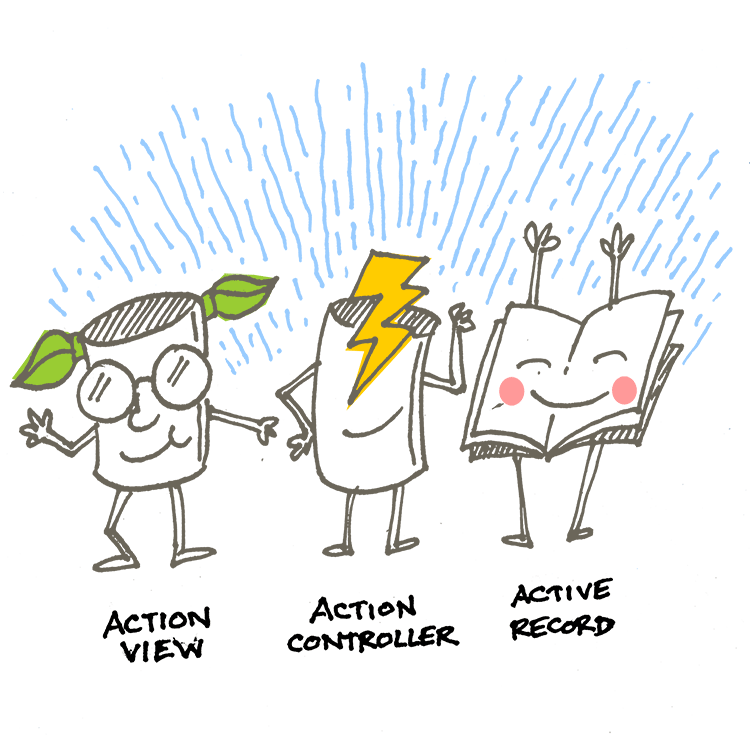
\includegraphics{src/img/action-pack.png}

\hypertarget{css-et-javascript}{%
\subsection{CSS et JavaScript}\label{css-et-javascript}}

\begin{itemize}
\tightlist
\item
  \begin{otherlanguage}{english}\texttt{foundation-rails}\end{otherlanguage}
\item
  \begin{otherlanguage}{english}\texttt{bootstrap-sass,\ \textasciitilde{}\textgreater{}\ 3.3.7}\end{otherlanguage}
\item
  \begin{otherlanguage}{english}\texttt{bootstrap,\ \textasciitilde{}\textgreater{}\ 4.0.0.alpha6}\end{otherlanguage}
\item
  \begin{otherlanguage}{english}\texttt{basscss-rails}\end{otherlanguage}
\item
  \begin{otherlanguage}{english}\texttt{bulma-rails}\end{otherlanguage}
\item
  \begin{otherlanguage}{english}\texttt{mui-sass}\end{otherlanguage}
\item
  etc.
\end{itemize}

Voir \href{http://guides.rubyonrails.org/asset_pipeline.html}{Asset
Pipeline}

Rails 5.1 proposera de gérer ces éléments-là via webpack ou yarn. D'ici
là, il nous faut passer par les gems associées.

\hypertarget{actioncable}{%
\subsection{ActionCable}\label{actioncable}}

La nouveauté de Rails 5.0.

Gestion simplifiée des
\begin{otherlanguage}{english}\texttt{WebSocket}\end{otherlanguage}
permettant d'incorporer des fonctionnalités « temps-réel ».

Voir
\href{http://guides.rubyonrails.org/action_cable_overview.html}{Action
Cable Overview}

\hypertarget{activejob}{%
\subsection{ActiveJob}\label{activejob}}

Gestion des tâches de fond, comme envoyer des e-mails, redimensionner
des images, \ldots{}

Voir \href{http://guides.rubyonrails.org/active_job_basics.html}{Active
Jobs Basics}

\hypertarget{actionview}{%
\subsection{ActionView}\label{actionview}}

La bonne méthode pour créer des formulaires et les lier à des données.

\begin{otherlanguage}{english}

\begin{verbatim}
<%= form_for @article, url: {action: 'create'} do |f| %>
  <%= f.text_field :title %>
  <%= f.submit 'Create' %>
<% end %>
\end{verbatim}

\end{otherlanguage}

Voir \href{http://guides.rubyonrails.org/form_helpers.html}{Form
Helpers}

\hypertarget{probluxe8me-avec-ruby-on-rails}{%
\section{Problème avec Ruby on
Rails}\label{probluxe8me-avec-ruby-on-rails}}

\includegraphics{src/img/microservices-demo.png}

\hypertarget{conclusion}{%
\section{Conclusion}\label{conclusion}}

\begin{itemize}
\tightlist
\item
  Laravel tire son inspiration première de Ruby on Rails.
\item
  Rails est plus cohérent dans son ensemble tirant partie des
  fonctionnalités de Ruby.
\end{itemize}

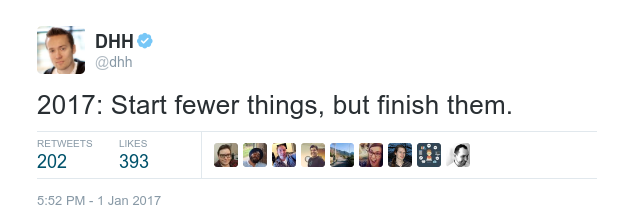
\includegraphics{src/img/dhh.png}(1)

\hypertarget{difficultuxe9s-pour-vous}{%
\subsection{Difficultés pour vous}\label{difficultuxe9s-pour-vous}}

\begin{itemize}
\tightlist
\item
  Construisez un produit au fur et à mesure
\item
  Déployez souvent
\item
  Essayer des bibliothèques
\item
  Et ayez un plan!
\end{itemize}


\includegraphics{src/img/rainbow.jpg}

\begin{otherlanguage}{english}

\end{otherlanguage}

\hypertarget{sources}{%
\section*{Sources}\label{sources}}
\addcontentsline{toc}{section}{Sources}

\hypertarget{refs}{}
\leavevmode\hypertarget{ref-dhh:2017}{}%
1. HEINEMEIER HANSSON, David. 2017: Start fewer things, but finish them.
{[}en~ligne{]}. 2017. {[}Consulté~le~7~février~2017{]}. Disponible à
l'adresse~: \url{https://twitter.com/dhh/status/815601578329575424}
